\section{实验五:Copy on write}\label{sec:Copy_on_write}

实现写时复制。

\subsection{实验目的}

\begin{enumerate}
	\item 理解什么是 Copy On Write(COW),其思想和作用是什么。
	\item 熟悉简单 fork() 系统调用的工作机制,提出一种 COW 的实现手段。
	\item 理解 xv6 中的 fork 函数,并修改内核程序,实现 COW。
\end{enumerate}

\subsection{实验内容}

修改 xv6 内核代码,使系统支持 Copy on Write 功能。

\begin{enumerate}
	\item 了解 Unix 中的 fork() 系统调用的功能以及实现机制,重点了解调用 fork()
	过程中的内存分配流程。
	\item 阅读 xv6 源码,理解 fork 函数以及父子进程拷贝内容的机制。
	\item 根据提示中给出的方案啊,修改 xv6 内核使系统支持 COW。
\end{enumerate}

\subsection{实验准备}

\subsubsection{控制台输入}

console.c 是 xv6 的控制台驱动程序,负责管理和处理来自用户的输入,它通过 UART(通用异步收发传输器)串口硬件接收用户键入的字符,驱动程序会累积一行输入,并处理特殊字符(如 backspace、Ctrl-u 等),保证用户输入的可编辑性。

xv6中使用的UART是QEMU模拟的16550芯片。UART硬件对于进程来说是一组memory-mapped寄存器,即RISC-V上有一些物理地址是直接和UART设备相连的。UART的地址从0x10000000或 \texttt{UART0} 开始,主要寄存器有:

\begin{enumerate}
	\item LSR寄存器(line status register):用来指示输入的字节是否准备好被用户进程读取。
	
	\item RHR寄存器(receive holding register):用来放置可以被用户进程读取的字节。当RHR中的一个字节被读取时,UART硬件将其从内部的FIFO硬盘中删除,当FIFO中为空时,LSR寄存器被置0。
	
	\item THR寄存器(transmit holding register):当用户进程向THR写入一个字节时,UART将传输这个字节。
\end{enumerate}

输入流程:

\begin{enumerate}
	\item 用户在 shell 输入字符,字符通过 UART 进入 CPU,产生中断。
	\item xv6 的 trap handler 进入 \texttt{devintr},判断是 UART 中断后,调用 \texttt{uartintr}。
	\item \texttt{uartintr} 读取 UART 的 RHR,获取字符,传递给 \texttt{consoleintr}。
	\item \texttt{consoleintr} 判断字符类型(如回车、退格),普通字符会 echo 回用户并存入 cons.buf。
	\item 输入一行结束(如回车)后,唤醒等待输入的 consoleread,数据被复制到用户空间。
\end{enumerate}

RISC-V对中断的支持:

\begin{enumerate}
	\item SIE寄存器(supervisor interrupt enable):用来控制中断,其中有一位是控制外部设备的中断(SEIE),一位控制suffer interrupt(一个CPU向另外一个CPU发出中断)(SSIE),一位控制定时器中断(STIE)
	
	\item SSTATUS寄存器(supervisor status):对某一个特定的CPU核控制是否接收寄存器,在kernel/riscv.h中的 \texttt{intr\_on} 被设置
	
	\item SIP寄存器(supervisor interrupt pending):观察这个寄存器来判断有哪些中断在pending
\end{enumerate}

\subsubsection{控制台输出}

UART 的输出缓冲区如 \cref{lst:URAT_output} 所示,包含写指针、读指针、锁保护。

\begin{listing}[!htb]
	\begin{minted}{c}
struct spinlock uart_tx_lock;
#define UART_TX_BUF_SIZE 32
char uart_tx_buf[UART_TX_BUF_SIZE];
uint64 uart_tx_w; // write next to uart_tx_buf[uart_tx_w % UART_TX_BUF_SIZE]
uint64 uart_tx_r; // read next from uart_tx_buf[uart_tx_r % UART_TX_BUF_SIZE]
	\end{minted}
	\caption{URAT 的输出缓冲区}\label{lst:URAT_output}
\end{listing}

在连接到控制台的文件描述符上执行 \texttt{write} 系统调用,最终将到达 \texttt{uartputc}(kernel/uart.c) 。设备驱动程序维护一个输出缓冲区(uart\_tx\_buf),这样写进程就不必等待UART完成发送;相反,\texttt{uartputc} 将每个字符附加到缓冲区,调用 \texttt{uartstart} 来启动设备传输(如果还未启动),然后返回。导致 \texttt{uartputc} 等待的唯一情况是缓冲区已满。

每当UART发送完一个字节,它就会产生一个中断。\texttt{uartintr} 调用 \texttt{uartstart},检查设备是否真的完成了发送,并将下一个缓冲的输出字符交给设备。因此,如果一个进程向控制台写入多个字节,通常第一个字节将由 \texttt{uartputc} 调用 \texttt{uartstart} 发送,而剩余的缓冲字节将由 \texttt{uartintr}调用 \texttt{uartstart} 发送,直到传输完成中断到来。

\subsubsection{定时器中断}

定时器中断是Xv6实现多任务处理的核心机制,其主要作用有维持系统时钟,切换进程和时间片轮转。

RISC-V要求定时器中断在机器模式而不是管理模式下进行。RISC-V机器模式无需分页即可执行,并且有一组单独的控制寄存器,因此在机器模式下运行普通的xv6内核代码是不实际的。因此,xv6处理定时器中断完全不同于上面列出的陷阱机制。

机器模式下执行的代码位于 kernrl/start.c 的 \texttt{timerinit} 中,它设置了接收定时器中断。工作的一部分是对CLINT(core-local interruptor)硬件编程,以在特定延迟后生成中断。另一部分是设置一个scratch区域,类似于trapframe,以帮助定时器中断处理程序保存寄存器和CLINT寄存器的地址。最后,\texttt{start}将 \texttt{mtvec} 设置为 \texttt{timervec},并使能定时器中断。

计时器中断可能发生在用户或内核代码正在执行的任何时候;内核无法在临界区操作期间禁用计时器中断。因此,计时器中断处理程序必须保证不干扰中断的内核代码。基本策略是处理程序要求RISC-V发出“软件中断”并立即返回。RISC-V用普通陷阱机制将软件中断传递给内核,并允许内核禁用它们。处理由定时器中断产生的软件中断的代码可以在 kernel/trap.c 的 \texttt{devintr} 中看到。

机器模式定时器中断向量是 kernel/kernelvec.S:93 的 \texttt{timervec}。它在 \texttt{start} 准备的scratch区域中保存一些寄存器,以告诉CLINT何时生成下一个定时器中断,要求RISC-V引发软件中断,恢复寄存器,并且返回。定时器中断处理程序中没有C代码。

\subsubsection{fork 系统调用}

在一个 Unix-like 的操作系统中,一个进程创建新进程的唯一方法是通过系统调用 fork。若是一个进程想要(并发地)执行一个新的程序,它应该先调用 fork 创建一个子进程,之后在子进程中使用 exec 系统调用来覆盖之后的行为。

fork 系统调用会拷贝当前进程的所有内存内容,创建一个只有 PID 和 PPID 与原来进程不一样的新进程。原进程被称作“父进程”,而新的进程被称作“子进程”。

在一个有效的 fork() 实现中,并不是所有父进程的内存空间/页面(在分页式内存管理中)都需要被拷贝。有以下两点原因: 

\begin{enumerate}
	\item 多数情况下,子进程都会通过 exec 覆盖父进程之后的程序体,父进程所拥有的程序、数据等占用内存空间的地方使用率不高。 
	
	\item 只有在父进程或者子进程修改了原有的数据后,才有必要对这一块内存进行拷贝。如果不做写入(write)而只是读取(read),并没有必要复制,父子进程间只要共享这个区域的内存就可以。
\end{enumerate}

\cref{lst:fork_uvmcopy} 通过函数 \texttt{uvmcopy} 复制了用户空间的所有页表。如果 \texttt{uvmcopy} 并不复制页面,而是将父子进程的页面关联(共享),并标记成只读状态,在写该页时就会发生一个缺页中断。针对缺页中断在 \texttt{usertrap} 函数中处理中断,为进程分配页面就能实现 COW 的主体功能。
在这样的解决方案之下存在另一个需要解决的问题:页面状态的记录与释放。Fork 调用产生的进程可能拥有自己修改过的页面(有 PTE\_W 标记的页面),或是与父进程共享一个页面(只有 PTE\_R 标记的页面)。在实现 COW 功能时需要正确地分配、记录和释放子进程产生的页面。
另外,xv6 提供了一个 copyout 函数以便用户将内存空间从内核拷贝到用户空间,这个函数也需要处理遇到 COW 页面的情况。

\begin{listing}[!htb]
	\begin{minted}{c}
// Copy user memory from parent to child.
if(uvmcopy(p->pagetable, np->pagetable, p->sz) < 0){
    freeproc(np); 
    release(&np->lock); 
    return -1;
}
	\end{minted}
	\caption{fork 函数部分片段}\label{lst:fork_uvmcopy}
\end{listing}

\subsection{实验过程}

\subsubsection{实现COW}

\begin{enumerate}
	\item 在 kernel/riscv.h中选取PTE中的保留位定义标记一个页面是否为COW Fork页面的标志位,如\cref{lst:define_PTE_COW} 所示。
	
	\item 在 kernel/kalloc.c中,定义引用计数的全局变量 \texttt{ref},包含一个自旋锁和引用计数数组。在 \texttt{kinit} 中初始化自旋锁,如\cref{lst:define_ref_and_init_self_lock} 所示。
	
	\item 修改 \texttt{freerange} 函数,将引用数设置为 1,否则在 \texttt{free} 中会被减为负数,如\cref{lst:change_freerange} 所示。
	
	\item 修改 \texttt{kalloc} 和 \texttt{kfree} 函数,在 \texttt{kalloc} 中初始化内存引用计数为1,在 \texttt{kfree} 中对内存引用计数减1,如果引用计数为0时才真正删除,如\cref{lst:change_kalloc_and_kfree} 所示。
	
	\item 添加 \texttt{krefcnt} 和 \texttt{kaddrefcnt} 函数,\texttt{krefcnt} 用于获取内存的引用计数,\texttt{kaddrefcnt} 用于增加内存的引用计数,如\cref{lst:krefcnt_and_kaddrefcnt} 所示。
	 
	\item 添加 \texttt{cowpage} 函数,用于判断一个页面是否是COW页面,如\cref{lst:cowpage} 所示。
	
	\item 添加 \texttt{cowalloc} 函数,用于实现 COW 分配,如\cref{lst:cowalloc} 所示。
	
	\item 修改 \texttt{uvmcopy} 函数,不为子进程分配内存,而是使父子进程共享内存,但禁用 \texttt{PTE\_W},同时标记 \texttt{PTE\_F},并调用 
	\texttt{kaddrefcnt} 增加引用计数,如\cref{lst:change_uvmcopy} 所示。
	
	\item 修改 \texttt{usertrap} 函数,处理页面错误,如\cref{lst:change_usertrap} 所示。
	
	\item 修改 \texttt{copyout} 函数,如\cref{lst:change_copyout} 所示
\end{enumerate}


\begin{listing}[!htb]
	\begin{minted}{c}
#define PTE_COW (1L << 8)
	\end{minted}
	\caption{定义是否为COW的标志位}\label{lst:define_PTE_COW}
\end{listing}

\begin{listing}[!htb]
	\begin{minted}{c}
struct ref_stru {
    struct spinlock lock;
    int cnt[PHYSTOP / PGSIZE];  // 引用计数
} ref;

void
kinit()
{
    initlock(&kmem.lock, "kmem");
    initlock(&ref.lock, "ref");
    freerange(end, (void*)PHYSTOP);
}
	\end{minted}
	\caption{定义ref并初始化自旋锁}\label{lst:define_ref_and_init_self_lock}
\end{listing}

\begin{listing}[!htb]
	\begin{minted}{c}
void
freerange(void *pa_start, void *pa_end)
{
    char *p;
    p = (char*)PGROUNDUP((uint64)pa_start);
    for(; p + PGSIZE <= (char*)pa_end; p += PGSIZE) {
        ref.cnt[(uint64)p / PGSIZE] = 1;
        kfree(p);
    }
}
	\end{minted}
	\caption{修改 freerange 函数}\label{lst:change_freerange}
\end{listing}

\begin{listing}[!htb]
	\begin{minted}{c}
void *
kalloc(void)
{
    struct run *r;
    
    acquire(&kmem.lock);
    r = kmem.freelist;
    if(r) {
        kmem.freelist = r->next;
        acquire(&ref.lock);
        ref.cnt[(uint64)r / PGSIZE] = 1;  // 将引用计数初始化为1
        release(&ref.lock);
    }
    release(&kmem.lock);
    
    if(r)
    memset((char*)r, 5, PGSIZE); // fill with junk
    return (void*)r;
}

void
kfree(void *pa)
{
    struct run *r;
    
    if(((uint64)pa % PGSIZE) != 0 || (char*)pa < end || (uint64)pa >= PHYSTOP)
    panic("kfree");
    
    acquire(&ref.lock);
    if(--ref.cnt[(uint64)pa / PGSIZE] == 0) {
        release(&ref.lock);
    
        r = (struct run*)pa;
    
        // Fill with junk to catch dangling refs.
        memset(pa, 1, PGSIZE);
       
        acquire(&kmem.lock);
        r->next = kmem.freelist;
        kmem.freelist = r;
        release(&kmem.lock);
    } else {
        release(&ref.lock);
    }
}
	\end{minted}
	\caption{修改 kalloc 和 kfree 函数}\label{lst:change_kalloc_and_kfree}
\end{listing}

\begin{listing}[!htb]
	\begin{minted}{c}
int krefcnt(void* pa) {
    return ref.cnt[(uint64)pa / PGSIZE];
}

int kaddrefcnt(void* pa) {
    if(((uint64)pa % PGSIZE) != 0 || (char*)pa < end || (uint64)pa >= PHYSTOP)
        return -1;
    acquire(&ref.lock);
    ++ref.cnt[(uint64)pa / PGSIZE];
    release(&ref.lock);
    return 0;
}
	\end{minted}
	\caption{添加 krefcnt 和 kaddrefcnt 函数}\label{lst:krefcnt_and_kaddrefcnt}
\end{listing}

\begin{listing}[!htb]
	\begin{minted}{c}
int 
cowpage(pagetable_t pagetable, uint64 va) {
    if(va >= MAXVA)
        return -1;
    pte_t* pte = walk(pagetable, va, 0);
    if(pte == 0)
        return -1;
    if((*pte & PTE_V) == 0)
        return -1;
    return (*pte & PTE_COW ? 0 : -1);
}
	\end{minted}
	\caption{添加 cowpage 函数}\label{lst:cowpage}
\end{listing}

\begin{listing}[!htb]
	\begin{minted}{c}
void* 
cowalloc(pagetable_t pagetable, uint64 va) {
    if(va % PGSIZE != 0)
    return 0;
    
    uint64 pa = walkaddr(pagetable, va);  // 获取对应的物理地址
    if(pa == 0)
        return 0;

    pte_t* pte = walk(pagetable, va, 0);  // 获取对应的PTE
    
    if(krefcnt((char*)pa) == 1) {
        // 只剩一个进程对此物理地址存在引用
        // 则直接修改对应的PTE即可
        *pte |= PTE_W;
        *pte &= ~PTE_COW;
        return (void*)pa;
    } else {
        // 多个进程对物理内存存在引用
        // 需要分配新的页面,并拷贝旧页面的内容
        char* mem = kalloc();
        if(mem == 0)
            return 0;
        
        // 复制旧页面内容到新页
        memmove(mem, (char*)pa, PGSIZE);
        
        // 清除PTE_V,否则在mappagges中会判定为remap
        *pte &= ~PTE_V;
        
        // 为新页面添加映射
        if(mappages(pagetable, va, PGSIZE, (uint64)mem, (PTE_FLAGS(*pte) | PTE_W) & ~PTE_COW) != 0) {
            kfree(mem);
            *pte |= PTE_V;
            return 0;
        }
        
        kfree((char*)PGROUNDDOWN(pa));
        return mem;
    }
}
	\end{minted}
	\caption{添加 cowalloc 函数}\label{lst:cowalloc}
\end{listing}

\begin{listing}[!htb]
	\begin{minted}{c}
int
uvmcopy(pagetable_t old, pagetable_t new, uint64 sz)
{
    pte_t *pte;
    uint64 pa, i;
    uint flags;

    for(i = 0; i < sz; i += PGSIZE){
        if((pte = walk(old, i, 0)) == 0)
            panic("uvmcopy: pte should exist");
        if((*pte & PTE_V) == 0)
            panic("uvmcopy: page not present");
        pa = PTE2PA(*pte);
        flags = PTE_FLAGS(*pte);

        // 仅对可写页面设置COW标记
        if(flags & PTE_W) {
            // 禁用写并设置COW Fork标记
            flags = (flags | PTE_COW) & ~PTE_W;
            *pte = PA2PTE(pa) | flags;
        }

        if(mappages(new, i, PGSIZE, pa, flags) != 0) {
            uvmunmap(new, 0, i / PGSIZE, 1);
            return -1;
        }
        // 增加内存的引用计数
        kaddrefcnt((char*)pa);
    }
    return 0;
}
	\end{minted}
	\caption{修改 uvmcopy 函数}\label{lst:change_uvmcopy}
\end{listing}

\begin{listing}[!htb]
	\begin{minted}{c}
void
usertrap(void)
{
    ...
    if(r_scause() == 8){
         ...
    } else if((which_dev = devintr()) != 0){
        // ok
    } else if(r_scause()  == 13 || r_scause()  == 15) {
        uint64 fault_va = r_stval();  // 获取出错的虚拟地址
        if(fault_va >= p->sz
        || cowpage(p->pagetable, fault_va) != 0
        || cowalloc(p->pagetable, PGROUNDDOWN(fault_va)) == 0)
        p->killed = 1;
    } else {
        printf("usertrap(): unexpected scause %p pid=%d\n", r_scause(), p->pid);
        printf("            sepc=%p stval=%p\n", r_sepc(), r_stval());
        p->killed = 1;
    }
    ...
}
	\end{minted}
	\caption{修改 usertrap 函数}\label{lst:change_usertrap}
\end{listing}

\begin{listing}[!htb]
	\begin{minted}{c}
int
copyout(pagetable_t pagetable, uint64 dstva, char *src, uint64 len)
{
    uint64 n, va0, pa0;
    
    while(len > 0){
        va0 = PGROUNDDOWN(dstva);
        pa0 = walkaddr(pagetable, va0);
        
        if(cowpage(pagetable, va0) == 0) {
            pa0 = (uint64)cowalloc(pagetable, va0);
        }

        if(pa0 == 0)
            return -1;
        ...
    }
    return 0;
}
	\end{minted}
	\caption{修改 copyout 函数}\label{lst:change_copyout}
\end{listing}

\begin{figure}[!htb]
	\centering
	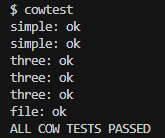
\includegraphics[width=0.4\textwidth]{test_cow}
	\caption{测试COW}
	\label{fig:test_cow}
\end{figure}

\begin{figure}[!htb]
	\centering
	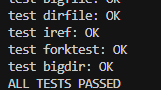
\includegraphics[width=0.5\textwidth]{test_cow_usertests}
	\caption{测试usertests2}
	\label{fig:test_cow_usertests}
\end{figure}

\subsubsection{综合测试}

在xv6-labs-2021目录下创建一个time.txt文件,记录我完成该lab花费的时间,使用\texttt{make grade}对lab5进行综合测试,测试通过。

\begin{figure}[!htb]
	\centering
	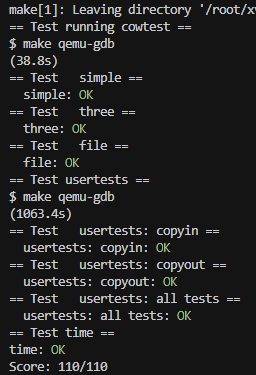
\includegraphics[width=0.5\textwidth]{test_lab5}
	\caption{lab5综合测试}
	\label{fig:test_lab5}
\end{figure}

\subsection{实验小结}